\chapter{Testování}
\label{testing}

Cílem testování v~této kapitole je zjistit výkonnost jednotlivých platforem a~porovnat je vůči sobě. 
Testy jsou zaměřeny primárně na měření časů průběhu hlavní smyčky při určitých činnostech tak, aby bylo možné srovnat výkonnost a~stabilitu jednotlivých platforem. 
Stabilitou je v~tomto případě myšlen rozdíl mezi průměrným a~maximálním naměřeným časem průchodu smyčky v~rámci opakovaných měření a~jednotlivých průchodů.

Při předchozí práci s~\EVthree{ } se systémem \evThreeDev (viz kapitola~\ref{lego-ev3dev}), že minimální perioda hlavní smyčky s~pár příkazy na vyčtení dat ze senzoru a následného nastavení motorů dle těchto hodnot (klasický program na jízdu po čáře) není kratší než 10~ms. 
Vzhledem k~výkonu procesoru (32bitový ARM na 300~MHz) v~\EVthree{ }je tento čas velmi zarážející. 

O~to větší překvapení nastalo, když jsem srovnával průměrnou periodu s~maximální. Ukázalo se, že ačkoliv je průměrná perioda přibližně 20~ms, maximální perioda může dosahovat až~100~ms. 
Takto velký rozptyl je pro potřeby regulace velmi problematický. 
Ve většině případů je potřeba mít konstantní čas průchodu hlavní smyčkou, aby rozdíl v~časech periody neovlivňoval měření a~následné řízení. 

Pokud bude nutné zajistit stabilní periodu, je třeba softwarově zpomalit průběh hlavní smyčky na maximální naměřený čas. 
Jedině tak lze zajistit konstantní periodu. 
Když by se použil tento postup, dostali bychom se na frekvenci 10~Hz, což je z~pohledu regulace již velmi nepříznivá hodnota.

Tyto testy byly provedeny na velmi jednoduchém programu. 
V případě rozsáhlejších projektů, kde by se pracovalo s~více vlákny a~periferiemi, mohou být výsledky ještě horší.

Proto jsem chtěl provést testování s~ekvivalentními programy na jednotlivých platformách a~zjistit, jestli tyto neduhy některá z~nich neodstraňuje a~za jakých situací k podobným problémům dochází.

\section{Forma testování}

Na počátku jsem zvažoval dvě formy testování. První počítala s~rozsáhlejší metodikou, v~rámci které bych testoval různé funkce \EVthree{}~\brick{{\it u}} a~zjišťoval, kde mohou být nejproblémovější místa z~pohledu výkonu. \\

V~rámci testů jsem se chtěl zaměřit na několik oblastí: % a jejich kombinace.

\begin{itemize}
	\item matematické operace
	\item čtení senzorů
	\item řízení motorů
\end{itemize}  

Tuto variantu jsem na počátku odložil, abych zkusil najít metodu jednoduší na implementaci a replikaci na jiné platformy. Následně v ní ale pokračuji v další části kapitoly.

Druhá varianta měla zajistit co možná nejstejnoměrnější podmínky měření času tak, aby jej neovlivňovalo fungování jednotlivých platforem. 
Proto mělo být k měření využito Arduino Uno a~velmi jednoduchý program  (příklad programu ve standardním prostředí pro \EVthree{ }na obrázku \ref{fig:LoopTimeLEDblinking-measuring}).
Program by jen blikal s dvěma LED\footnote{LED = Light-Emitting Diode –- dioda emitující světlo} (zelenou a červenou) umístěnými na přední straně pod ovládacími tlačítky na \EVbrick{{\it u}} a~čas svitu jednotlivých LED by měřilo Arduino.

%U jednotlivých platforem by se měřili časy průchodů hlavní smyčkou a z těchto naměřených dat by se vytvářeli histogramy pro následné vyhodnocení.

% Následně jsem se ale rozhodl pro jinou strategii testování. 
% Rozhodl jsem se ale pro jinou strategii testování. 

% Po čase jsem tuto strategii zavrhl. 

Jednalo by se totiž o~jeden z~nejlepších způsobů, jak demonstrovat problémy s~dobou trvání jednotlivých cyklů a~práci s periferiemi. 
V~optimálním případě by totiž měla kombinací těchto dvou barevných LED vzniknout oranžová. 

Pokud by se tak nestalo, pozorovatel by měl hned optickou zpětnou vazbu a~zároveň lze jednoduše měřit časové prodlevy mezi spínáním a~vypínáním jednotlivých LED pomocí měřicí sestavy s Arduinem.

\section{Měření pomocí LED}


\begin{figure}[h]
	\centering
	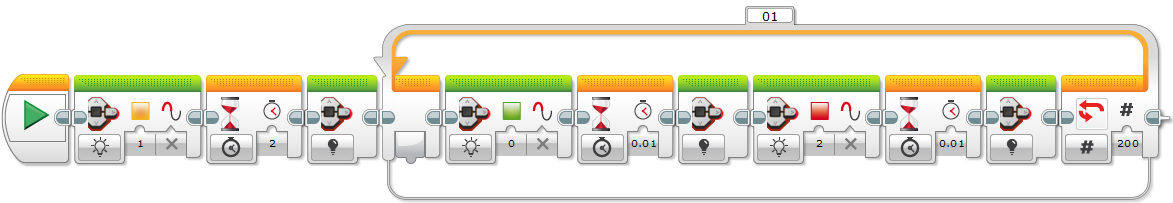
\includegraphics[width=\textwidth]{images/measuring-ev3-software_LoopTimeLEDblinking.png}
	\caption[Ukázka jednoduchého programu na blikání zelenou a červenou LED]{Ukázka jednoduchého programu na blikání zelenou a červenou LED}
	\label{fig:LoopTimeLEDblinking-measuring}
\end{figure}

Ukázkový program je připraven tak, že každá LED se vždy rozsvítí na 10~ms ($T~=~0.01~s~= 10~ms$), následně zhasne a~rozsvítí se druhá LED. 

Celkový čas jednoho průchodu cyklem trvá 20~ms ($T~=~T_{LED1}~+ T_{LED2}$) a~frekvence blikání by měla být 50~Hz ($f~=~\frac{1}{T}~= \frac{1}{0.02~s} =~50~Hz$). 
Což je frekvence, kterou již lidské oko nezaznamená (filmy mají standardní frekvenci obnovování snímku 24 až 30~Hz). % TODO: a běžné televizní vysílání má 50~Hz).
Celkový počet opakování hlavní smyčky je zvolen na 200. 
Blikání má tedy probíhat 4~sekundy ($t~=~T~\cdot~counter =~0.02~ms~\cdot~200~= 4~s$).

Pro měřicí sestavu byl vybrán fototranzistor BPX~81\footnote{\url{http://cz.rs-online.com/web/p/fototranzistory/6655255/}} (má velmi široké rozpětí vstupních vlnových délek -- zvládne viditelné i~infra světlo) s~Arduinem Uno (viz obrázek~\ref{fig:arduino-measuring-system}). \\

Tato kombinace mi přijde nejvhodnější z~několika důvodů: 

\begin{itemize}
	\item velmi rozšířený hardware (Arduino Uno)
	\item rychlé sestavení
	\item možnost snadného naprogramování
	\item jednoduchá duplikovatelnost (zopakování experimentu)
\end{itemize}  

Nejdůležitějším bodem pro tuto variantu byla jednoduchá duplikovatelnost, která umožňuje komukoliv provést stejná měření, ať už pro kontrolu v~této práci prezentovaných výsledků, nebo pro otestování jiné platformy a~porovnání s~naměřenými daty z~této práce.

\begin{figure}[h]
	\centering
	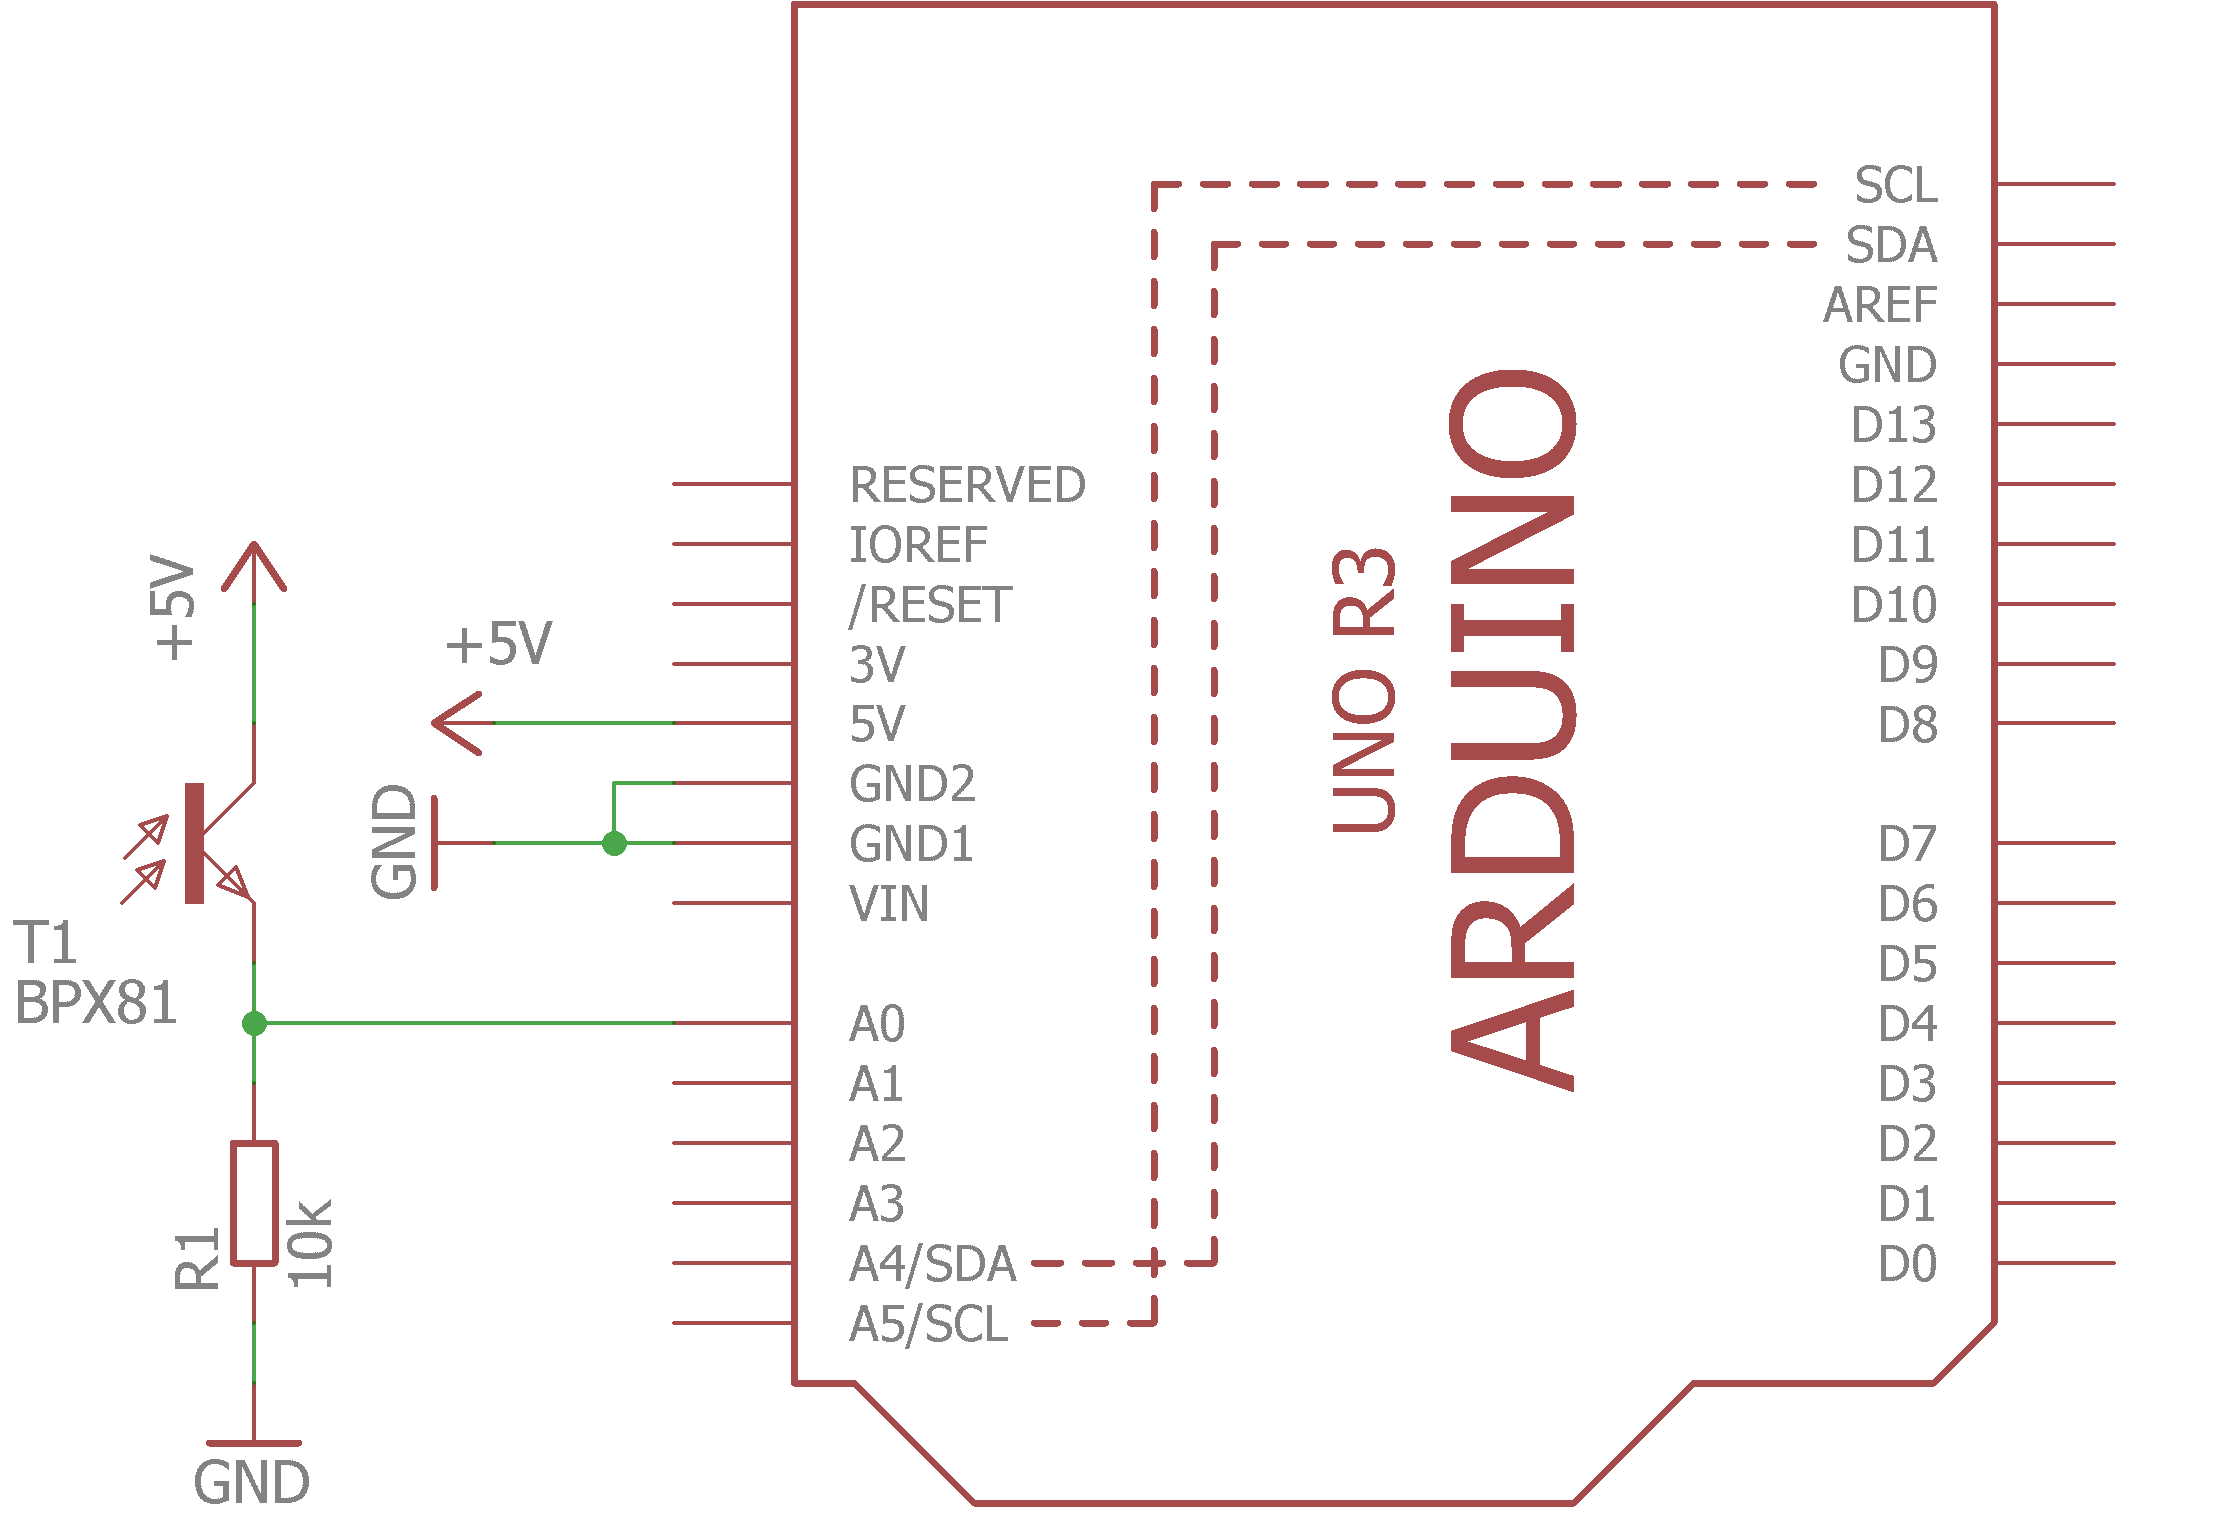
\includegraphics[width=250px]{images/measuring-arduino-system_schema.png}	
	\caption[Schéma zapojení měřicího systému]{Schéma zapojení měřicího systému}
	\label{fig:arduino-measuring-system}
\end{figure}

Jelikož se druhá varianta zdála vhodnější, otestoval jsem ji s~programem, prezentovaným výše, s~danou měřicí sestavou a~osciloskopem. 

\begin{figure}[h]
	\centering
	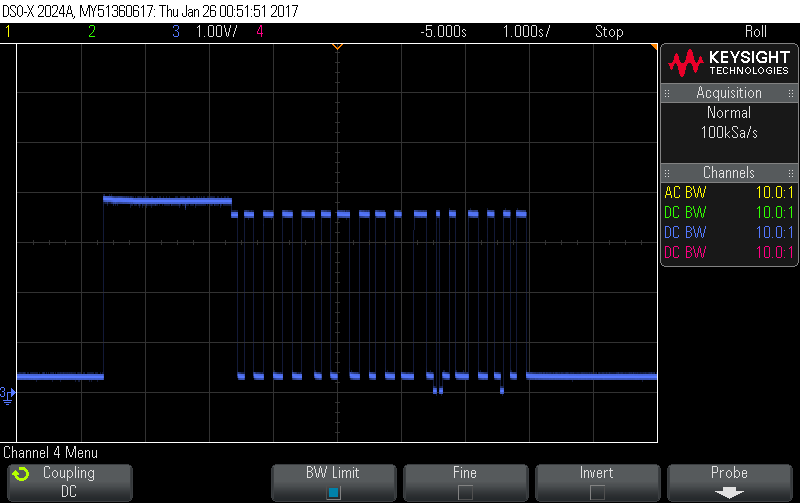
\includegraphics[width=350px]{images/measuring-oscilloscope_ev3-software_led-blinking_all.png}
	\caption[Záznam signálu z osciloskopu po provedení zkušebního programu]{Záznam signálu z osciloskopu po provedení zkušebního programu}
	\label{fig:measuring_lego-ev3_orig-soft_led-blinking_all}
\end{figure}

Výsledky byly velice překvapivé. Celkový počet pulzů červené LED (napětí na osciloskopu přibližně 3,7~V; pro zelenou 0,3~V; oranžová 3,9~V) byl 17 
(viz obrázek~\ref{fig:measuring_lego-ev3_orig-soft_led-blinking_all}). Přičemž dle programu mělo proběhnout 200~pulzů.  

Při detailním zkoumání se ukázalo, že LED nedokáží blikat na 50~Hz, ale mohou svůj stav měnit vždy s~frekvencí 20~Hz. 
Každých 50~ms docházelo ke kontrole stavových proměnných u~LED a~případné změně stavu (viz~obrázek~\ref{fig:measuring_lego-ev3_orig-soft_led-blinking_part1} -- jeden dílek odpovídá 100~ms a~1~V).

Toto chování lze například vysvětlit tak, že v~rámci operačního systému \EVbrick{\it u} je v určité periodě (přibližně 50~ms) vyvoláno přerušení od časovače, které porovná stav proměnných a~registrů LED a~dle výsledku buď rozsvítí, nebo zhasne. 
Proto v~daných intervalech dochází k~interferenci mezi časováním LED (20~ms) a~interního přerušení (přibližně 50~ms) a~podle toho, jak se tyto události sejdou, se jednotlivé LED přepínají.
Tento časovač bude pravděpodobně fungovat jen pro LED, ale nebude dále ovlivňovat další chování systému.
 
\begin{figure}[h]
	\centering
	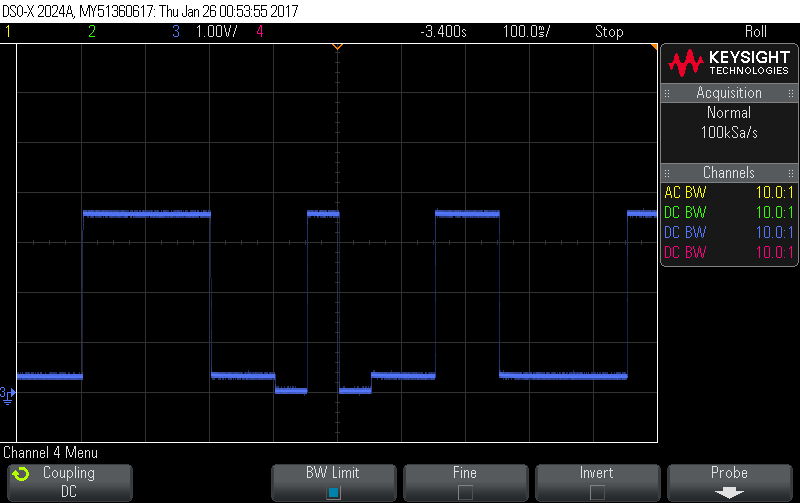
\includegraphics[width=350px]{images/measuring-oscilloscope_ev3-software_led-blinking_part1.png}
	\caption[Zoom na záznam z osciloskopu po provedení zkušebního programu]{Zoom na záznam z osciloskopu po provedení zkušebního programu}
	\label{fig:measuring_lego-ev3_orig-soft_led-blinking_part1}
\end{figure}

\begin{figure}[h]
	\centering
	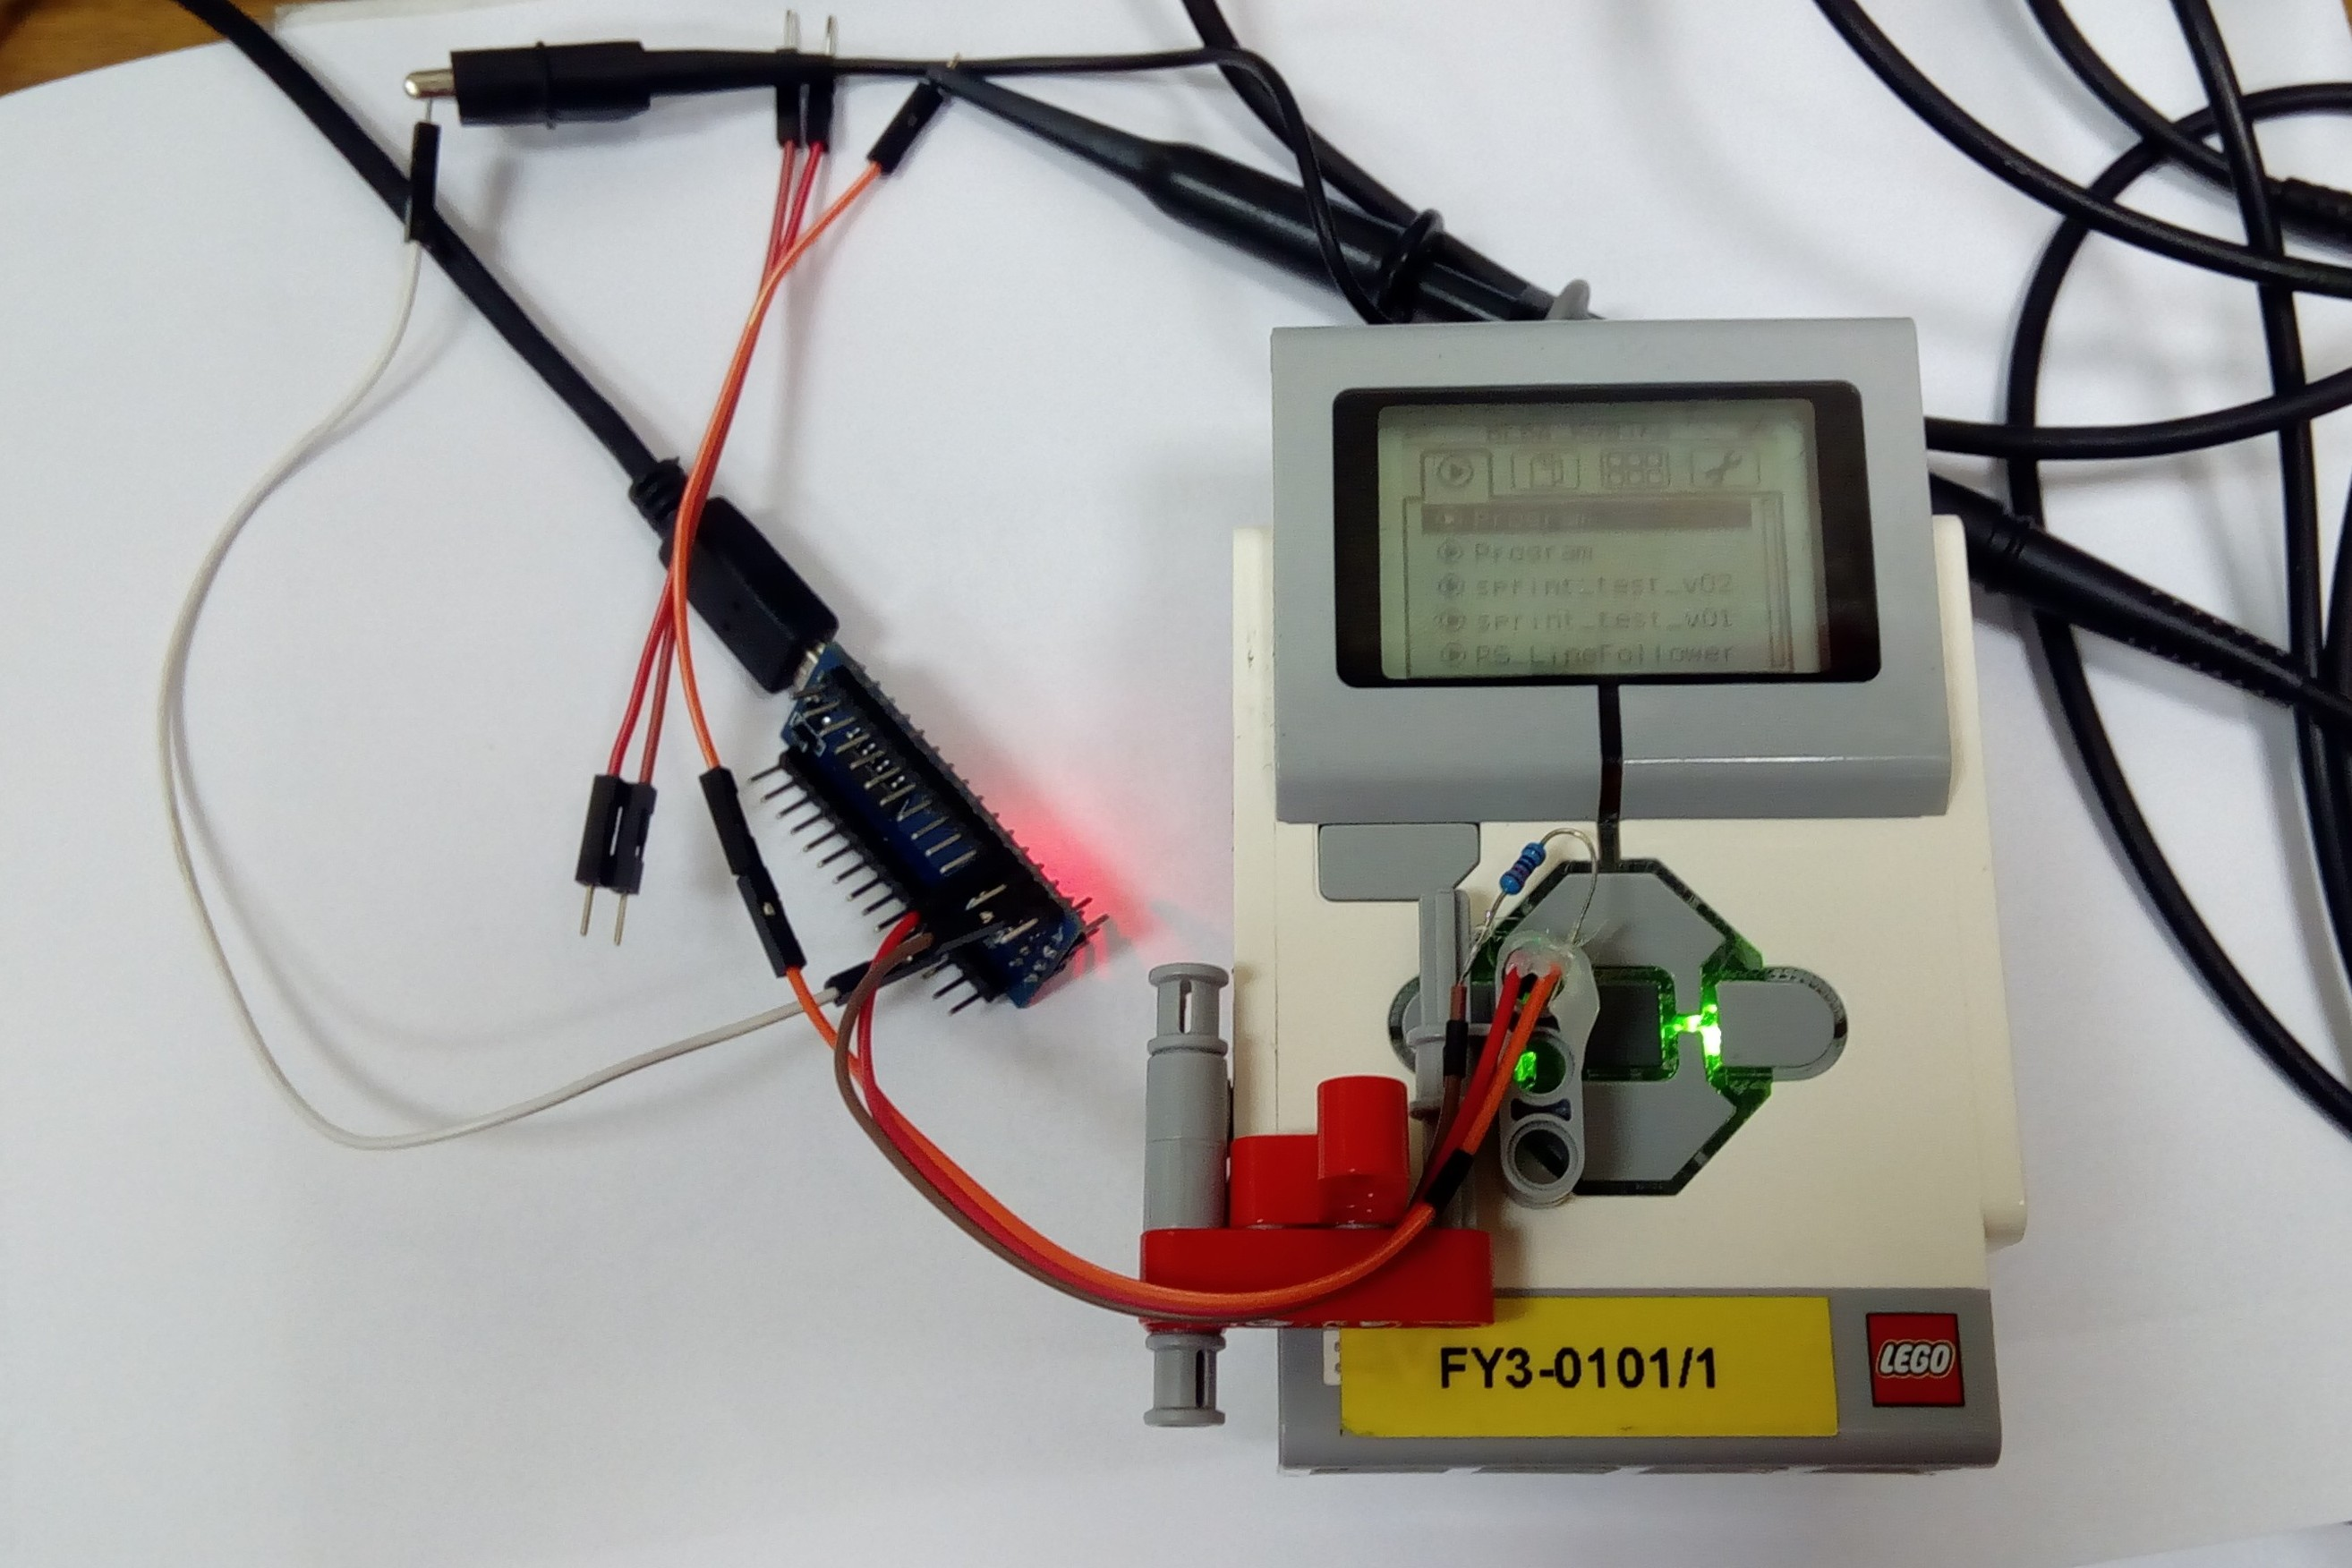
\includegraphics[width=280px]{images/measuring-system_photo.jpg}
	\caption[Foto měřicí sestavy]{Foto měřicí sestavy}
	\label{fig:measuring-system_photo}
\end{figure}

Z~naměřených výsledků vyplývá, že tuto formu testování nelze použít.

\section{Měření jednotlivých operací}

Jelikož nebyli výsledky z~prvního testování uspokojivé, rozhodl jsem se provést testy výkonosti jednotlivých operací na standardním LEGO systému a~RTOS EV3RT (popis v~kapitole \ref{lego-EV3RT}), který dle předchozího zkoumání měl předpoklady k nejlepšímu výkonu.  \\

V rámci testů byla vytvořeny dvě sady: 

\begin{itemize}
    \item matematických operací (sčítání, násobení, dělení, \dots) a~podmínka
    \item operace se senzory a motory
\end{itemize}

Jednotlivé měření se prováděli vícenásobným voláním daných metod (v~rozmezí od~1 do~100~000 volání v závislosti na době trvání dané operace) tak, aby bylo možné změřit čas s rozumnou přesností.
Každé měření pak bylo zopakováno 1000, aby bylo možné určit průměr a maxima. 
Zdrojové soubory k testům (jak LEGO, tak EV3RT) jsou k dispozici v repozitáři RB-ev3rt-hrp2-sdk~\cite{RB-ev3rt-hrp2-sdk-github}.

Matematické operace, jako sčítání, násobení, dělení byly prováděny v plovoucí desetinné čárce (double).

Z~výkonnostních testu (tabulka~\ref{Benchmark-math} a~\ref{Benchmark-IO}) je dobře vidět, že zpracování operací probíhá na systému EV3RT více jak o~2~řády rychlejší než u~oficiálního systému \EVthree{}. Proto jsem vybral tento systém jako nejvhodnější variantu pro  vytvoření vývojové prostředí.

\begin{table}[h]
\centering

\caption{Porovnání relativního výpočetního výkonu originálního LEGO systému a~EV3RT -- matematické operace a podmínka \\
}

\label{Benchmark-math}
\begin{tabular}{@{}ccrrr@{}}
\toprule
Označení testu                                       & AVG/MAX                     & LEGO                               & EV3RT                                & Porovnání                                                    \\ \midrule
\multicolumn{1}{|c}{}                                & \cellcolor[HTML]{EFEFEF}AVG & \cellcolor[HTML]{EFEFEF}    563 us & \cellcolor[HTML]{EFEFEF}    0.586 us & \multicolumn{1}{r|}{\cellcolor[HTML]{EFEFEF}    960 $\times$}  \\
\multicolumn{1}{|c}{\multirow{-2}{*}{sčítání}}           & \cellcolor[HTML]{FFFFFF}MAX & \cellcolor[HTML]{FFFFFF}    680 us & \cellcolor[HTML]{FFFFFF}    0.602 us & \multicolumn{1}{r|}{\cellcolor[HTML]{FFFFFF}   1129 $\times$}  \\ \midrule
\multicolumn{1}{|c}{}                                & \cellcolor[HTML]{EFEFEF}AVG & \cellcolor[HTML]{EFEFEF}    388 us & \cellcolor[HTML]{EFEFEF}    0.506 us & \multicolumn{1}{r|}{\cellcolor[HTML]{EFEFEF}    766 $\times$}  \\
\multicolumn{1}{|c}{\multirow{-2}{*}{násobení}}          & \cellcolor[HTML]{FFFFFF}MAX & \cellcolor[HTML]{FFFFFF}    510 us & \cellcolor[HTML]{FFFFFF}    0.526 us & \multicolumn{1}{r|}{\cellcolor[HTML]{FFFFFF}    969 $\times$}  \\ \midrule
\multicolumn{1}{|c}{}                                & \cellcolor[HTML]{EFEFEF}AVG & \cellcolor[HTML]{EFEFEF}    403 us & \cellcolor[HTML]{EFEFEF}    2.627 us & \multicolumn{1}{r|}{\cellcolor[HTML]{EFEFEF}    153 $\times$}  \\
\multicolumn{1}{|c}{\multirow{-2}{*}{dělení}}           & \cellcolor[HTML]{FFFFFF}MAX & \cellcolor[HTML]{FFFFFF}    510 us & \cellcolor[HTML]{FFFFFF}    2.943 us & \multicolumn{1}{r|}{\cellcolor[HTML]{FFFFFF}    173 $\times$}  \\ \midrule
\multicolumn{1}{|c}{}                                & \cellcolor[HTML]{EFEFEF}AVG & \cellcolor[HTML]{EFEFEF}    557 us & \cellcolor[HTML]{EFEFEF}   43.350 us & \multicolumn{1}{r|}{\cellcolor[HTML]{EFEFEF}     12 $\times$}  \\
\multicolumn{1}{|c}{\multirow{-2}{*}{mocnina}}           & \cellcolor[HTML]{FFFFFF}MAX & \cellcolor[HTML]{FFFFFF}   1480 us & \cellcolor[HTML]{FFFFFF}   47.860 us & \multicolumn{1}{r|}{\cellcolor[HTML]{FFFFFF}     30 $\times$}  \\ \midrule
\multicolumn{1}{|c}{}                                & \cellcolor[HTML]{EFEFEF}AVG & \cellcolor[HTML]{EFEFEF}    488 us & \cellcolor[HTML]{EFEFEF}    5.250 us & \multicolumn{1}{r|}{\cellcolor[HTML]{EFEFEF}     92 $\times$}  \\
\multicolumn{1}{|c}{\multirow{-2}{*}{odmocnina}}          & \cellcolor[HTML]{FFFFFF}MAX & \cellcolor[HTML]{FFFFFF}    890 us & \cellcolor[HTML]{FFFFFF}    6.146 us & \multicolumn{1}{r|}{\cellcolor[HTML]{FFFFFF}    144 $\times$}  \\ \midrule
\multicolumn{1}{|c}{}                                & \cellcolor[HTML]{EFEFEF}AVG & \cellcolor[HTML]{EFEFEF}    411 us & \cellcolor[HTML]{EFEFEF}   12.520 us & \multicolumn{1}{r|}{\cellcolor[HTML]{EFEFEF}     32 $\times$}  \\
\multicolumn{1}{|c}{\multirow{-2}{*}{sinus}}           & \cellcolor[HTML]{FFFFFF}MAX & \cellcolor[HTML]{FFFFFF}    590 us & \cellcolor[HTML]{FFFFFF}   15.780 us & \multicolumn{1}{r|}{\cellcolor[HTML]{FFFFFF}     37 $\times$}  \\ \midrule
\multicolumn{1}{|c}{}                                & \cellcolor[HTML]{EFEFEF}AVG & \cellcolor[HTML]{EFEFEF}    419 us & \cellcolor[HTML]{EFEFEF}    0.126 us & \multicolumn{1}{r|}{\cellcolor[HTML]{EFEFEF}   3325 $\times$}  \\
\multicolumn{1}{|c}{\multirow{-2}{*}{podmínka}}     & \cellcolor[HTML]{FFFFFF}MAX & \cellcolor[HTML]{FFFFFF}    510 us & \cellcolor[HTML]{FFFFFF}    0.139 us & \multicolumn{1}{r|}{\cellcolor[HTML]{FFFFFF}   3669 $\times$}  \\ \midrule
\end{tabular}
\end{table}

\begin{table}[]
\centering
\caption{Porovnání relativního výpočetního výkonu originálního LEGO systému a~EV3RT -- \brick{} komponenty, motory a senzory}
\label{Benchmark-IO}
\begin{tabular}{@{}ccrrr@{}}
\toprule
Označení testu                                       & AVG/MAX                     & LEGO                               & EV3RT                                & Porovnání                                                    \\ \midrule
\multicolumn{1}{|c}{}                                & \cellcolor[HTML]{EFEFEF}AVG & \cellcolor[HTML]{EFEFEF}    966 us & \cellcolor[HTML]{EFEFEF}    0.350 us & \multicolumn{1}{r|}{\cellcolor[HTML]{EFEFEF}   2760 $\times$}  \\
\multicolumn{1}{|c}{\multirow{-2}{*}{brick button}}  & \cellcolor[HTML]{FFFFFF}MAX & \cellcolor[HTML]{FFFFFF}   1100 us & \cellcolor[HTML]{FFFFFF}    0.362 us & \multicolumn{1}{r|}{\cellcolor[HTML]{FFFFFF}   3038 $\times$}  \\ \midrule
\multicolumn{1}{|c}{}                                & \cellcolor[HTML]{EFEFEF}AVG & \cellcolor[HTML]{EFEFEF}    787 us & \cellcolor[HTML]{EFEFEF}    2.866 us & \multicolumn{1}{r|}{\cellcolor[HTML]{EFEFEF}    274 $\times$}  \\
\multicolumn{1}{|c}{\multirow{-2}{*}{brick led}}     & \cellcolor[HTML]{FFFFFF}MAX & \cellcolor[HTML]{FFFFFF}    900 us & \cellcolor[HTML]{FFFFFF}    3.247 us & \multicolumn{1}{r|}{\cellcolor[HTML]{FFFFFF}    277 $\times$}  \\ \midrule
\multicolumn{1}{|c}{}                                & \cellcolor[HTML]{EFEFEF}AVG & \cellcolor[HTML]{EFEFEF}   1449 us & \cellcolor[HTML]{EFEFEF}  396.080 us & \multicolumn{1}{r|}{\cellcolor[HTML]{EFEFEF}      3 $\times$}  \\
\multicolumn{1}{|c}{\multirow{-2}{*}{brick display}} & \cellcolor[HTML]{FFFFFF}MAX & \cellcolor[HTML]{FFFFFF}   1620 us & \cellcolor[HTML]{FFFFFF}  409.330 us & \multicolumn{1}{r|}{\cellcolor[HTML]{FFFFFF}      3 $\times$}  \\ \midrule
\multicolumn{1}{|c}{}                                & \cellcolor[HTML]{EFEFEF}AVG & \cellcolor[HTML]{EFEFEF}    603 us & \cellcolor[HTML]{EFEFEF}    8.770 us & \multicolumn{1}{r|}{\cellcolor[HTML]{EFEFEF}     68 $\times$}  \\
\multicolumn{1}{|c}{\multirow{-2}{*}{motor power}}   & \cellcolor[HTML]{FFFFFF}MAX & \cellcolor[HTML]{FFFFFF}    720 us & \cellcolor[HTML]{FFFFFF}   11.630 us & \multicolumn{1}{r|}{\cellcolor[HTML]{FFFFFF}     61 $\times$}  \\ \midrule
\multicolumn{1}{|c}{}                                & \cellcolor[HTML]{EFEFEF}AVG & \cellcolor[HTML]{EFEFEF}    612 us & \cellcolor[HTML]{EFEFEF}    8.840 us & \multicolumn{1}{r|}{\cellcolor[HTML]{EFEFEF}     69 $\times$}  \\
\multicolumn{1}{|c}{\multirow{-2}{*}{motor speed}}   & \cellcolor[HTML]{FFFFFF}MAX & \cellcolor[HTML]{FFFFFF}    760 us & \cellcolor[HTML]{FFFFFF}   11.670 us & \multicolumn{1}{r|}{\cellcolor[HTML]{FFFFFF}     65 $\times$}  \\ \midrule
\multicolumn{1}{|c}{}                                & \cellcolor[HTML]{EFEFEF}AVG & \cellcolor[HTML]{EFEFEF}   1023 us & \cellcolor[HTML]{EFEFEF}   17.490 us & \multicolumn{1}{r|}{\cellcolor[HTML]{EFEFEF}     58 $\times$}  \\
\multicolumn{1}{|c}{\multirow{-2}{*}{motors speed}}  & \cellcolor[HTML]{FFFFFF}MAX & \cellcolor[HTML]{FFFFFF}   1160 us & \cellcolor[HTML]{FFFFFF}   21.120 us & \multicolumn{1}{r|}{\cellcolor[HTML]{FFFFFF}     54 $\times$}  \\ \midrule
\multicolumn{1}{|c}{}                                & \cellcolor[HTML]{EFEFEF}AVG & \cellcolor[HTML]{EFEFEF}    785 us & \cellcolor[HTML]{EFEFEF}    3.870 us & \multicolumn{1}{r|}{\cellcolor[HTML]{EFEFEF}    202 $\times$}  \\
\multicolumn{1}{|c}{\multirow{-2}{*}{CS reflected}}  & \cellcolor[HTML]{FFFFFF}MAX & \cellcolor[HTML]{FFFFFF}    940 us & \cellcolor[HTML]{FFFFFF}    6.980 us & \multicolumn{1}{r|}{\cellcolor[HTML]{FFFFFF}    134 $\times$}  \\ \midrule
\multicolumn{1}{|c}{}                                & \cellcolor[HTML]{EFEFEF}AVG & \cellcolor[HTML]{EFEFEF}    830 us & \cellcolor[HTML]{EFEFEF}    3.860 us & \multicolumn{1}{r|}{\cellcolor[HTML]{EFEFEF}    215 $\times$}  \\
\multicolumn{1}{|c}{\multirow{-2}{*}{CS ambient}}    & \cellcolor[HTML]{FFFFFF}MAX & \cellcolor[HTML]{FFFFFF}    990 us & \cellcolor[HTML]{FFFFFF}    7.100 us & \multicolumn{1}{r|}{\cellcolor[HTML]{FFFFFF}    139 $\times$}  \\ \midrule
\multicolumn{1}{|c}{}                                & \cellcolor[HTML]{EFEFEF}AVG & \cellcolor[HTML]{EFEFEF}    799 us & \cellcolor[HTML]{EFEFEF}    3.890 us & \multicolumn{1}{r|}{\cellcolor[HTML]{EFEFEF}    205 $\times$}  \\
\multicolumn{1}{|c}{\multirow{-2}{*}{CS color}}      & \cellcolor[HTML]{FFFFFF}MAX & \cellcolor[HTML]{FFFFFF}    930 us & \cellcolor[HTML]{FFFFFF}    6.730 us & \multicolumn{1}{r|}{\cellcolor[HTML]{FFFFFF}    138 $\times$}  \\ \midrule
\multicolumn{1}{|c}{}                                & \cellcolor[HTML]{EFEFEF}AVG & \cellcolor[HTML]{EFEFEF}    811 us & \cellcolor[HTML]{EFEFEF}    3.841 us & \multicolumn{1}{r|}{\cellcolor[HTML]{EFEFEF}    211 $\times$}  \\
\multicolumn{1}{|c}{\multirow{-2}{*}{UTS cm}}        & \cellcolor[HTML]{FFFFFF}MAX & \cellcolor[HTML]{FFFFFF}    960 us & \cellcolor[HTML]{FFFFFF}    4.212 us & \multicolumn{1}{r|}{\cellcolor[HTML]{FFFFFF}    227 $\times$}  \\ \midrule
\multicolumn{1}{|c}{}                                & \cellcolor[HTML]{EFEFEF}AVG & \cellcolor[HTML]{EFEFEF}    827 us & \cellcolor[HTML]{EFEFEF}    3.838 us & \multicolumn{1}{r|}{\cellcolor[HTML]{EFEFEF}    215 $\times$}  \\
\multicolumn{1}{|c}{\multirow{-2}{*}{UTS inch}}      & \cellcolor[HTML]{FFFFFF}MAX & \cellcolor[HTML]{FFFFFF}   1030 us & \cellcolor[HTML]{FFFFFF}    4.197 us & \multicolumn{1}{r|}{\cellcolor[HTML]{FFFFFF}    245 $\times$}  \\ \midrule
\multicolumn{1}{|c}{}                                & \cellcolor[HTML]{EFEFEF}AVG & \cellcolor[HTML]{EFEFEF}    845 us & \cellcolor[HTML]{EFEFEF}    3.769 us & \multicolumn{1}{r|}{\cellcolor[HTML]{EFEFEF}    224 $\times$}  \\
\multicolumn{1}{|c}{\multirow{-2}{*}{UTS listen}}    & \cellcolor[HTML]{FFFFFF}MAX & \cellcolor[HTML]{FFFFFF}   1220 us & \cellcolor[HTML]{FFFFFF}    4.115 us & \multicolumn{1}{r|}{\cellcolor[HTML]{FFFFFF}    296 $\times$}  \\ \midrule
\multicolumn{1}{|c}{}                                & \cellcolor[HTML]{EFEFEF}AVG & \cellcolor[HTML]{EFEFEF}    851 us & \cellcolor[HTML]{EFEFEF}    3.910 us & \multicolumn{1}{r|}{\cellcolor[HTML]{EFEFEF}    217 $\times$}  \\
\multicolumn{1}{|c}{\multirow{-2}{*}{GYRO angle}}    & \cellcolor[HTML]{FFFFFF}MAX & \cellcolor[HTML]{FFFFFF}   1050 us & \cellcolor[HTML]{FFFFFF}    6.740 us & \multicolumn{1}{r|}{\cellcolor[HTML]{FFFFFF}    155 $\times$}  \\ \midrule
\multicolumn{1}{|c}{}                                & \cellcolor[HTML]{EFEFEF}AVG & \cellcolor[HTML]{EFEFEF}    847 us & \cellcolor[HTML]{EFEFEF}    3.920 us & \multicolumn{1}{r|}{\cellcolor[HTML]{EFEFEF}    216 $\times$}  \\
\multicolumn{1}{|c}{\multirow{-2}{*}{GYRO rate}}     & \cellcolor[HTML]{FFFFFF}MAX & \cellcolor[HTML]{FFFFFF}   1250 us & \cellcolor[HTML]{FFFFFF}    7.190 us & \multicolumn{1}{r|}{\cellcolor[HTML]{FFFFFF}    173 $\times$}  \\ \midrule
\multicolumn{1}{|c}{}                                & \cellcolor[HTML]{EFEFEF}AVG & \cellcolor[HTML]{EFEFEF}  25712 us & \cellcolor[HTML]{EFEFEF}    3.510 us & \multicolumn{1}{r|}{\cellcolor[HTML]{EFEFEF}   7325 $\times$}  \\
\multicolumn{1}{|c}{\multirow{-2}{*}{GYRO reset}}    & \cellcolor[HTML]{FFFFFF}MAX & \cellcolor[HTML]{FFFFFF}  34410 us & \cellcolor[HTML]{FFFFFF}    6.420 us & \multicolumn{1}{r|}{\cellcolor[HTML]{FFFFFF}   5359 $\times$}  \\ \midrule
\end{tabular}
\end{table}

